\section{Vine Overview}

\begin{figure}
\centering
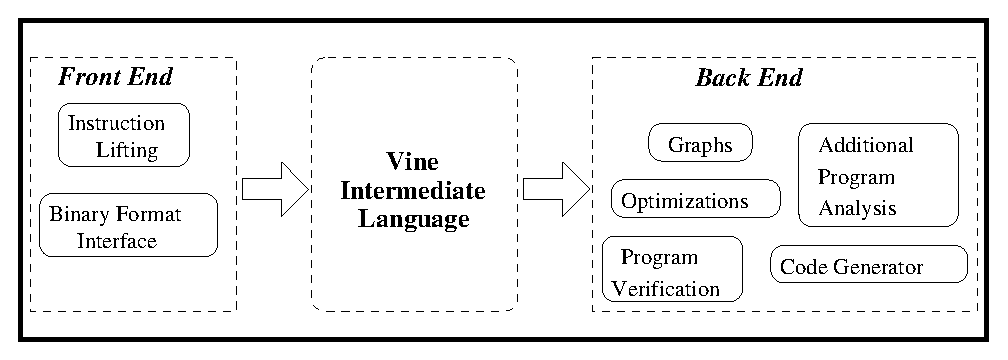
\includegraphics[width=.6\textwidth]{vine-components}
\caption{Vine Overview}
\label{fig:vine-components}
\end{figure}

Figure~\ref{fig:vine-components} shows a high-level picture of
Vine. The Vine static analysis component is divided into a
platform-specific front-end and a platform-independent back-end.  At
the core of Vine is a platform-independent intermediate language
(IL) for assembly.
Previously, we also used the name IR (intermediate representation)
for this language, and that abbreviation persists in some command and
option names, and as a file extension.
The IL is designed as a small and carefully
specified language that faithfully represents the assembly
languages. Assembly instructions in the underlying architecture are
translated to the Vine IL, a process we refer to as {\em lifting}, via
the Vine front-end.  All back-end
analyses are performed on the platform-independent IL. Thus, program
analyses can be written in an architecture-independent fashion and
do not need to directly deal with the complexity of an instruction
set such as x86. This design also provides extensibility---users can
easily write their own analysis on the IL by building on top of the
core utilities provided in Vine.

The Vine front-end currently supports translating 32-bit x86
to the IL. It uses a set of
third-party libraries to parse different binary formats and
produce assembly. The assembly is then translated into the Vine IL in
a syntax-directed manner.

The Vine back-end supports a variety of core program analysis
utilities.  The back-end has utilities for creating a variety of
different graphs, such as control flow and program dependence graphs.
The back-end also provides an optimization framework. The optimization
framework is usually used to simplify a specific set of
instructions. We also provide program verification capabilities such
as symbolic execution, calculating weakest preconditions, and
interfacing with decision procedures.  Vine can also write out lifted
Vine instructions as valid C code via the code generator back-end.

To combine static and dynamic analysis, we also provide an interface
for Vine to read an execution trace generated by a dynamic analysis
component such as TEMU. The execution trace can be lifted to the IL
for various further analysis.
